%% fundamentals.tex
%%

%------------------------------------------------------------------------------------------------
\section{Grundlagen}
\label{sec:Grundlagen}
%------------------------------------------------------------------------------------------------

Innerhalb dieses Kapitels werden zu Beginn die notwendige Nomenklatur für die Bestandteile des \ac{iot} und deren Funktion eingeführt. Im Anschluss an die Einführung in die Grundlagen bezüglich des Gebiets \ac{iot} werden die derzeit existierenden Regelwerke für die Bewertung der Einhaltung von Datensicherheit und Privatsphäre genauer betrachtet. Bezüglich der Definition von zu schützenswerten Informationen, werden basierend auf der folgenden Analyse die Variante der europäischen Rechtssprechung beschrieben. Abschließend erfolgt eine Auflistung von Gefahren, die resultierend aus ungemäßem Umgang mit \ac{pii} für den einzelnen Nutzer von \ac{iot}-Geräten entstehen kann.

%------------------------------------------------------------------------------------------------
\subsection{Geräte des \acl{iot}}
\label{sec:Grundlagen:sssec:Geräte des Internet of Things}
%------------------------------------------------------------------------------------------------

Beginnend mit der Definition eines Geräts aus dem Bereich \ac{iot}, oder auch kurz Smart Device. Diesbezüglich findet sich in der Literatur unterschiedlichste Arten von Interpretationen. Grundlegend gilt, dass innerhalb des \acs{iot} Geräte verschiedenster Art miteinander in Interaktion treten. Hierbei reicht die Bandbreite von Gadgets des alltäglichen Gebrauchs, u.a. Mobiltelefone oder Smart Watches, bis hin zu autonomen Robotern aus der Industrie 4.0, die über Kameras und Sensoren ihre Umwelt in Wechselwirkung treten \cite{Li2015}. Dies geschieht hierbei ohne jegliches Zutun eines Menschen über das Internet. Architektonisch lässt sich das \ac{iot} in drei Schichten unterteilen. Diese können basierend auf der Definition von \cite{Seliem2018} folgendermaßen darstellen:

\begin{itemize}
\item Die \textbf{Geräte-Schicht} (Device Layer) beschreibt hierbei die Schicht mit allen physikalischen Ressourcen, die Daten sammeln und regulieren. Diese Schicht beinhaltet somit die Grundgesamtheit aller heterogenen und ressourcenbeschränkten Geräte.
\item Die \textbf{Plattform-Schicht} (Platform Layer) repräsentiert die klassischen Netzwerk-Schicht (Network Layer) im OSI Modell. Diese Schicht integriert die notwendige Vorverarbeitung der Daten und reduziert somit die Anforderungen an die Ressourcen innerhalb der Applikation-Schicht.
\item Die \textbf{Applikation-Schicht} (Application Layer) setzt sich wiederum aus zwei Teilen zusammen. Auf der einen Seite die Unterstützungsschicht (Support Layer), auf der das Edge Computing und die analytischen Dienste laufen und auf der anderen Seite die Applikation-Dienst-Schicht (Application Service Layer), die die notwendige Unterstützung bezüglich der Rechenressourcen für die \ac{iot} Infrastruktur bereitstellt.
\end{itemize}

\begin{figure}
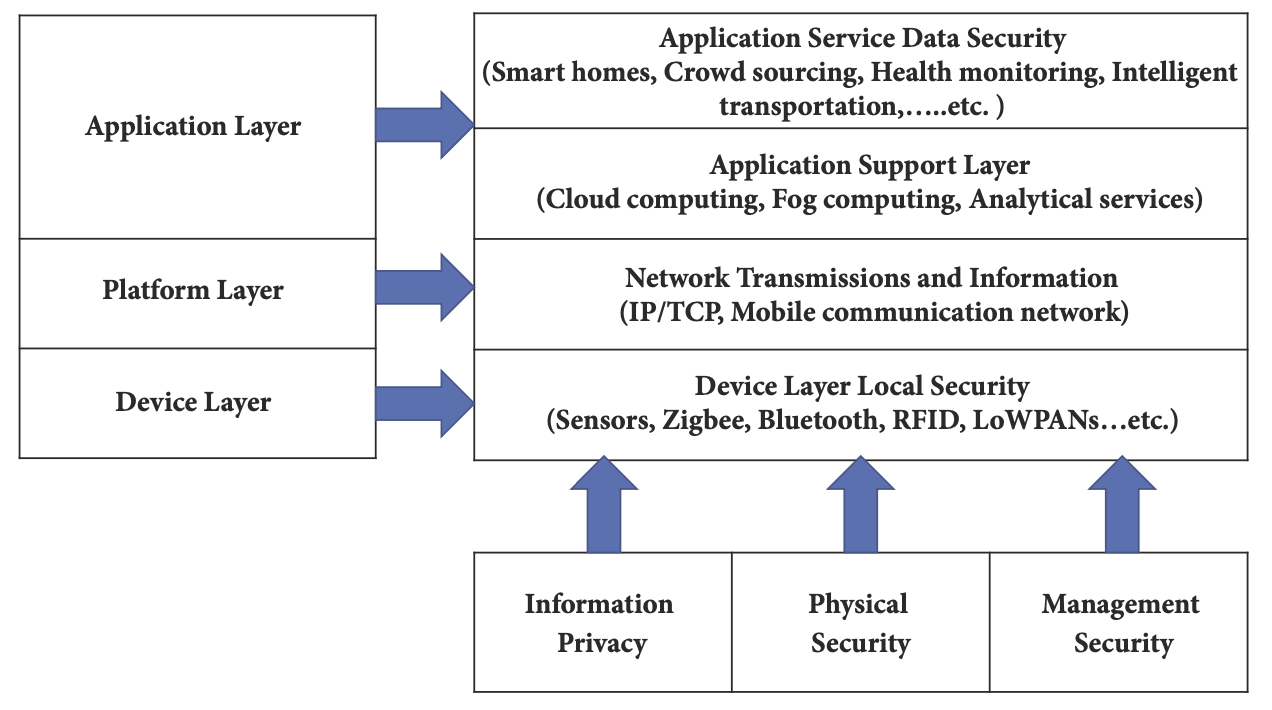
\includegraphics[width=\textwidth]{fundamentals/pictures/IoT_Layer_Architecture}
\caption{Drei Schichten Architektur des \ac{iot} zur Untergliederung der einzelnen Komponenten gemäß \cite{Seliem2018}}
\label{fig:drei-schichten-iot}
\end{figure}

Wie bereits in der Illustration \ref{fig:drei-schichten-iot} angedeutet, lassen die einzelnen Schichten eine feinere Unterteilung im Rahmen unterschiedlichster Nutzungsfälle zu. Beispielsweise werden in anderen Publikationen, diese Thematik betreffend, auch vier Schichten für eine genauere Unterteilung der einzelnen Bestandteile genutzt. Da dies als Teil dieser Ausarbeitung jedoch nicht relevant ist, werden auch im späteren Verlauf nur die Drei-Schicht-Modelle verwendet.

%------------------------------------------------------------------------------------------------
\subsection{Rechtliche Rahmenbedingungen}
\label{sec:Grundlagen:ssec:Rechtliche Rahmenbedingungen}
%------------------------------------------------------------------------------------------------

Der gesetzliche Kontext für die Regulation und Einhaltung der Datenschutzrichtlinien wird im europäischen Raum durch die \acl{gdpr} bzw. \acl{dsgvo}. Innerhalb dieses Regelwerkes werden die Akteure und deren Regeln und Pflichten im Umgang mit \ac{pii} und \ac{nonpii} beschrieben und somit sichergestellt, dass bestimmte Standards an Sicherheit und Privatsphäre länderübergreifend umgesetzt werden. Im Gegensatz zu dem klaren Rahmenwerk in der \ac{eu} existieren im angloamerikanischen Raum wiederum die Regeln der \acl{ftc}. Nachfolgend werden diese Rahmenwerke beziehungsweise Institutionen nochmals genauer beschrieben.

%------------------------------------------------------------------------------------------------
\subsubsection{\acl{gdpr}}
\label{sec:Grundlagen:ssec:Rechtliche Rahmenbedingungen:sssec:GDPR}
%------------------------------------------------------------------------------------------------

Durch Inkrafttreten der \ac{gdpr} / \ac{dsgvo} am 25.05.2018 wurde von der \acl{eu} ein einheitlicher Katalog an Regeln geschaffen, der den allgemeinen Umgang bezüglich der Erhebung und der Verarbeitung von Daten im europäischen Raum beschreibt. Ziel sind hierbei (global) Unternehmen und Einrichtungen, die innerhalb der \acl{eu} als Teil ihrer Dienstleistung Daten von \ac{eu}-Bürgern erheben und diese verarbeiten. Als Nachfolger der Data Protection Directive 95/46/EC löste sie diese mit der erstmaligen Einführung der \ac{gdpr} 2016/679 am 24.05.2016 bereits ab. Zweck dieses Rahmenwerkes war die Harmonisierung der Datenschutz- und Privatsphäre-Regelungen innerhalb der europäischen Union \cite{Bastos2019}.

Neben der Definition von zentralen Begrifflichkeiten und Eckpunkten stehen die Formulierung von Prinzipien im Mittelpunkt des Gesetzestextes. Zur Einordnung dieser, wird beginnend mit der nachfolgenden Auflistung ein Überblick über die beteiligten rechtlichen Entitäten auf Basis von \cite{DSGVOArt4} gegeben.

\begin{itemize}
\item \textbf{\acl{ds} / \textbf{betroffene Person} beschreibt eine natürliche Person im Kontext des jeweiligen Rechtsstaates.
\item \textbf{\acl{dc} / \textbf{Verantwortlicher} beschreibt eine natürliche oder rechtliche Person, die den Zweck und den Vorgang der Verarbeitung der persönlichen Daten definiert.
\item \textbf{\acl{dp} / \textbf{Auftragsverarbeiter} beschreibt eine natürliche oder rechtliche Person, die auf Anordnung des \textbf{Verantwortlichen} die persönlichen Daten verarbeitet.
\end{itemize}

Im späteren Verlauf dieser Arbeit werden für das bessere Verständnis nur noch die Abkürzungen der englischen Bezeichnungen für die Akteure verwendet. Darauf aufbauend stehen die Grundprinzipien der \ac{dsgvo} als Wegweiser für die Rechte dieser "Personen". Nachfolgend aufgelistet stehen die \textbf{sieben} Grundprinzipien, die im Rahmen der Datenverarbeitung durch \textbf{Verantwortliche} und \textbf{Auftragsverarbeiter} einzuhalten sind. Die Formulierungen sind anhand von \cite{DSGVOArt5} präzisiert worden:

\begin{itemize}
\item \textbf{Fair, lawful and transparent processing} / \textbf{Rechtmäßigkeit, Verarbeitung nach Treu und Glauben, Transparenz} \\ Die Verarbeitung von personenbezogenen Daten muss für die betroffene Person nachvollziehbar sein.
\item \textbf{Purpose Limitation} / \textbf{Zweckbindung} \\ Die Verarbeitung der personenbezogenen Daten darf nur im Rahmen des Zwecks der Erhebung geschehen.
\item \textbf{Data Minimisation} / \textbf{Datenminimierung} \\ Die Datenmenge muss dem Zweck angemessen und somit nur auf das notwendige Maß für die Verarbeitung beschränkt sein.
\item \textbf{Accuracy} / \textbf{Richtigkeit} \\ Die Daten müssen in korrekter Form vorliegen und auf dem aktuellen Stand gehalten werden. Alle nicht korrekten Einträge müssen gelöscht werden.
\item \textbf{Storage Limitation} / \textbf{Speicherbegrenzung} \\ Die Daten dürfen nur so lange gespeichert werden, wie es dem Zweck der Verarbeitung dient.
\item \textbf{Integrity and Confidentiality} / \textbf{Integrität und Vertraulichkeit} \\ Die Verarbeitung der Daten muss so gestaltet werden, dass ein bestimmtes Maß an Sicherheit gewährleistet werden kann, um unbefugten Zugriff oder Verlust zu vermeiden.
\item \textbf{Accountability} / \textbf{Rechenschaftspflicht} \\ Der \textbf{\ac{ac}} ist für die Einhaltung der obigen \textbf{sechs} Prinzipien verantwortlich und muss dies nachweisen können.
\end{itemize}

%------------------------------------------------------------------------------------------------
\subsubsection{\acl{ftc}}
\label{sec:Grundlagen:ssec:Rechtliche Rahmenbedingungen:sssec:FTC}
%------------------------------------------------------------------------------------------------

Im Vergleich zur \fullref{sec:Grundlagen:ssec:Rechtliche Rahmenbedingungen:sssec:GDPR} aus dem vorherigen Unterkapitel, steht bei der \acl{ftc) eine politische Institution hinter der Regulation der Datensicherheit und Privatsphäre in Amerika. Dabei kümmert sich die \ac{ftc} nicht nur ausschließlich um die Einhaltung von Datenschutz und Privatsphäre, sondern bedient auch andere Ressorts im Bereich des Schutzes der Öffentlichkeit vor nicht-rechtsmäßigen Geschäftsmethodiken. Hierbei umspannt der abdeckte Rahmen von der Beratung von Endkunden bezüglich Einkauf, Krediten und Identitätsdiebstahl bis hin zu Beratung im wirtschaftlichen Kontext. Somit beschreibt die \ac{ftc} nicht nur die Regeln, sondern kann diese auch effektiv umsetzen \cite{FTC}. Als gleichwertiges Organ kann hier die \textbf{\textit{Abteilung für Recht der Europäischen Kommission}} gesehen werden \cite{FTCEU}.

%------------------------------------------------------------------------------------------------
\subsection{Klassifikation von Daten}
\label{sec:Grundlagen:ssec:Klassifikation von Daten}
%------------------------------------------------------------------------------------------------

Wie bereits in \fullref{sec:Einleitung:ssec:Motivation} erwähnt, können die gesammelten Daten auf Basis ihres Informationsgehaltes in unterschiedliche Kategorien eingeteilt werden. Hierzu kann in die nachfolgenden Kategorien von \ac{pii} und \ac{nonpii} im gröbsten Sinne unterschieden werden. Bei genauerer Betrachtung können diese generalisierten Klassen weiter ausdifferenziert werden. Im Rahmen dieser Arbeit wird jedoch nur in die beiden genannten Arten unterschieden. Jede dieser Klassen besitzt neben der für sie einzigartigen Information einen anderen Anspruch an deren Schutz.

%------------------------------------------------------------------------------------------------
\subsubsection{\acf{pii}}
\label{sec:Grundlagen:ssec:Klassifikation von Daten:sssec:PII}
%------------------------------------------------------------------------------------------------
Die \ac{pii} beschreiben eine Information, die Daten enthält, die wiederum auf eine Person zurückgeführt werden können, von der die Daten gesammelt wurden. Die Gefahren, die mit dieser Art von Daten verbunden sind, werden im nachfolgenden Unterkapitel genauer beschrieben. Klassische Beispiele für \acs{pii} sind zum Beispiel:
\begin{itemize}
\item Vorname und Nachname
\item E-Mail Adresse
\item ...
\end{itemize}

%------------------------------------------------------------------------------------------------
\subsubsection{\acf{nonpii}}
\label{sec:Grundlagen:ssec:Klassifikation von Daten:sssec:Non-PII}
%------------------------------------------------------------------------------------------------

%------------------------------------------------------------------------------------------------
\subsection{Gefahren für die Privatsphäre}
\label{sec:Grundlagen:ssec:Gefahren für die Privatsphäre}
%------------------------------------------------------------------------------------------------

